%%% Local Variables: 
%%% coding: utf-8
%%% mode: latex
%%% TeX-engine: xetex
%%% End: 

\documentclass[hide notes,intlimits]{beamer}
\mode<presentation>
{
  \usetheme[footline]{PISMshade}
  \setbeamercovered{transparent}
}

% load packages
\usepackage{media9}
\usepackage[english]{babel}
\usepackage[multidot]{grffile}

\usepackage{tikz}
\usetikzlibrary{shapes,arrows}
\usetikzlibrary{shadows}

\definecolor{dark red}{HTML}{E41A1C}
\definecolor{dark green}{HTML}{4DAF4A}
\definecolor{dark violet}{HTML}{984EA3}
\definecolor{dark blue}{HTML}{084594}
\definecolor{dark orange}{HTML}{FF7F00}
\definecolor{light blue}{HTML}{377EB8}
\definecolor{light red}{HTML}{FB9A99}
\definecolor{light violet}{HTML}{CAB2D6}

\setbeamercolor{boxed}{fg=black,bg=light blue!25}
\graphicspath{{figures/}{../figures/}{../figures_2018_08/}{../2021_09_cph/figures/}{../2021_11_geo/figures/}}

\newenvironment{transbox}[1][]{%
\begin{tikzpicture}
\node[drop shadow,rounded corners,text width=.9\textwidth,fill=white, fill opacity=#1,text opacity=1] \bgroup
}{
\egroup;\end{tikzpicture}} 

\newenvironment{transbox-tight}{%
\begin{tikzpicture}
\node[drop shadow,rounded corners,fill=uaf yellow, fill opacity=0.75,text opacity=1] \bgroup
}{
\egroup;\end{tikzpicture}} 

\newcommand{\jl}{[\![}
\newcommand{\jr}{]\!\hskip 0.003cm ]}
\newcommand{\bpsi}{\boldsymbol{\psi}}
\newcommand{\bPsi}{\boldsymbol{\Psi}}
\newcommand{\bphi}{\boldsymbol{\phi}}
\newcommand{\bPhi}{\boldsymbol{\Phi}}
\newcommand{\bn}{\mathbf{n}}
\newcommand{\bq}{\mathbf{q}}
\newcommand{\bv}{\mathbf{v}}
\newcommand{\D}{\,\mathrm{d}}
\newcommand{\Tsnow}{T_{\text{snow}}}
\newcommand{\Hatm}{H_{\text l}^{\text{atm}}}

\newcommand{\mathtext}[1]{\mathsf{#1}}

% title page
\title[Ice sheet modeling] % (optional, use only with long paper titles)
{Predicting sea-level rise from ice sheets}
\subtitle{The Good, the Bad, and the Ugly}
\author[Aschwanden] % (optional, use only with lots of authors)
{\textbf{Andy Aschwanden}\\ with \\D. Brinkerhoff, M. Truffer, T. Bartholomaus}
\institute{Geophysical Institute, University of Alaska Fairbanks}

% - Give the names in the same order as the appear in the paper.
% - Use the \inst{?} command only if the authors have different
%   affiliation.

% - Use the \inst command only if there are several affiliations.
% - Keep it simple, no one is interested in your street address.
 \titlegraphic{\vskip-.5cm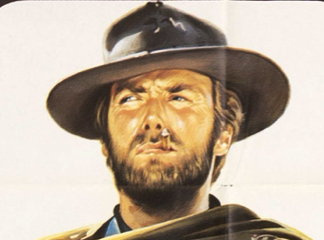
\includegraphics[height=1.5cm]{thegood}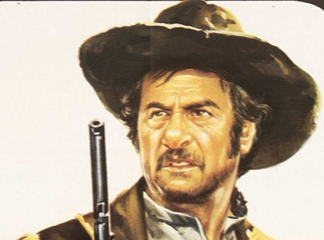
\includegraphics[height=1.5cm]{thebad}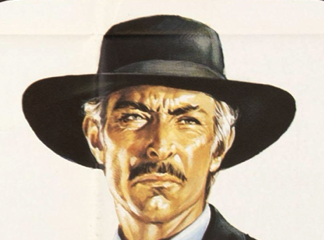
\includegraphics[height=1.5cm]{theugly}}

\date{}


\subject{Credible sea-level projections}

\begin{document}



\setbeamertemplate{background canvas}
  {
     \tikz{\node[inner sep=0pt,opacity=0.6] {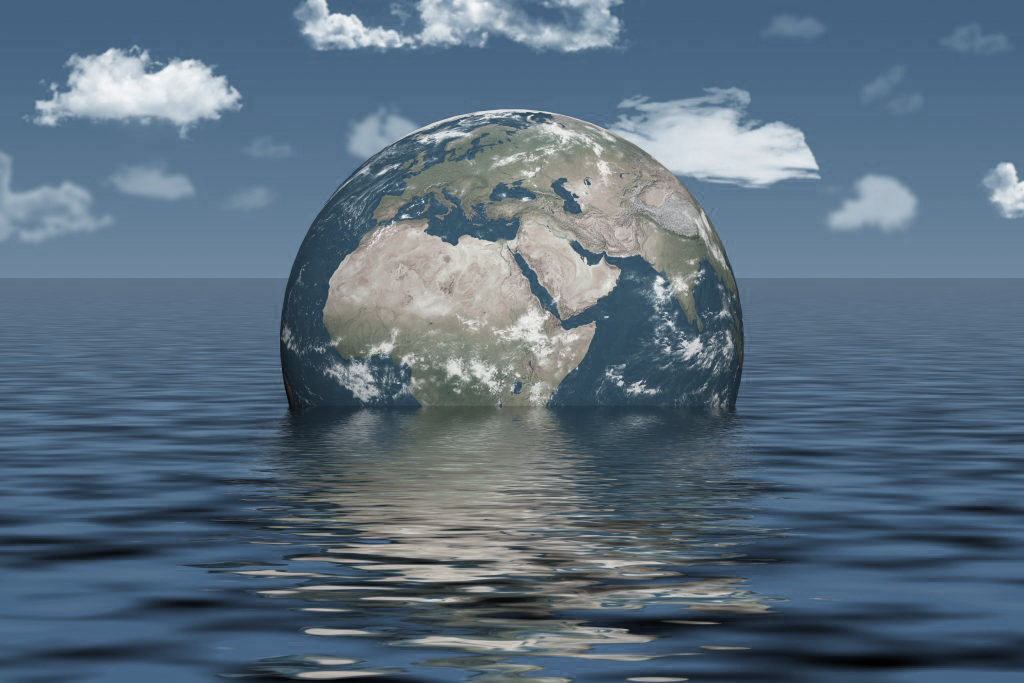
\includegraphics[height=\paperheight]{earth-drowning-desat}};}
}


 
% insert titlepage
\begin{frame}
  \titlepage
  \note[item]{Collaboration Martin, Doug, Tim}
\end{frame}

\setbeamertemplate{background canvas}
  {
}


\begin{frame}{How this talk came about}
  \begin{figure}
    \includegraphics<1>[width=.9\textwidth]{ar6_wg1_fig_9_17_draft_with_zoom}
    \caption{IPCC AR6 Draft, Fig. 9.17}
  \end{figure}
\end{frame}


\begin{frame}
  \frametitle{Questions}
  \begin{itemize}
  \item What is going on?
  \item How did we get here?
  \item How can we move forward?
  \end{itemize}
\end{frame}

\part{How did we get here?}
\frame{\partpage}


\begin{frame}
  \frametitle{The 1990s}
      \begin{figure}
        \includegraphics<1>[width=\textwidth]{greve-1995}
      \end{figure}
\end{frame}

\begin{frame}
  \frametitle{The 1990s}
      \vspace{-2em}
  \begin{columns}[c]
    \begin{column}{.5\linewidth}
    \begin{figure}
        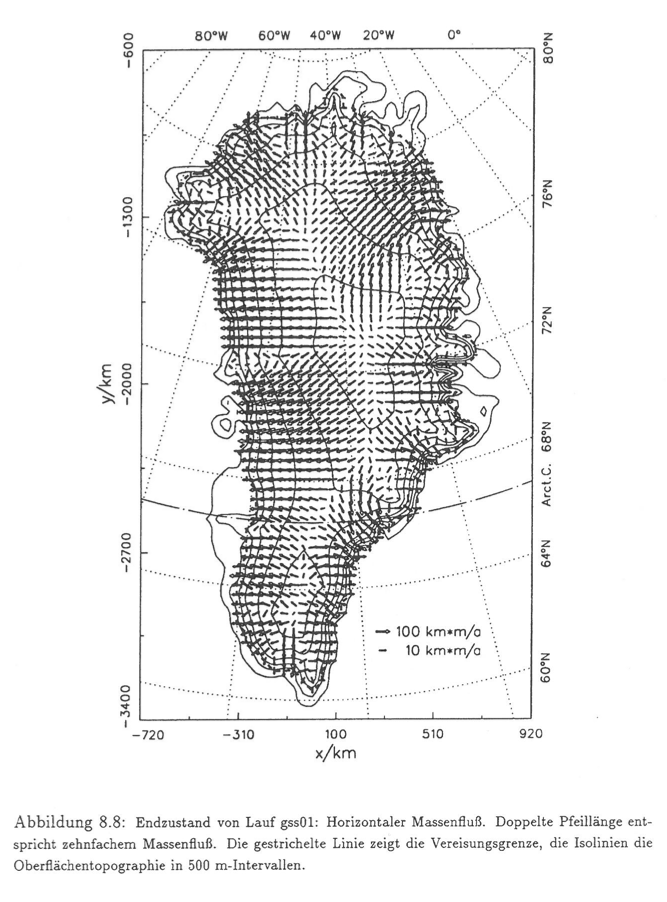
\includegraphics[height=0.75\textheight]{greve_1995_flow}
    \end{figure}
    \end{column}
    \begin{column}{.4\linewidth}
      \begin{figure}
      \includegraphics[height=.7\textheight]{greenland-obs-rignot}
      \caption{\tiny{Rignot \& Mouginot, 2012}}
      \end{figure}
    \end{column}
  \end{columns}
\end{frame}


\begin{frame}
  \frametitle{IPCC AR3, 2001}
  \begin{columns}[c]
    \begin{column}{.4\linewidth}
      \begin{figure}
        \includegraphics[height=5cm]{ar3-wg1}
      \end{figure}
    \end{column}
    \begin{column}{.5\linewidth}
      \begin{itemize}
        \item 1 ice sheet model (?)
        \item ``The Antarctic ice sheet is likely to gain mass, while the Greenland ice sheet is likely to lose mass''
        \item ``However, loss of grounded ice leading to substantial sea level rise from WAIS is now widely agreed to be very unlikely during the 21st century''
      \end{itemize}
    \end{column}
\end{columns}
\end{frame}


\begin{frame}
  \frametitle{IPCC AR4, 2007}
  \begin{columns}[c]
    \begin{column}{.4\linewidth}
      \begin{figure}
        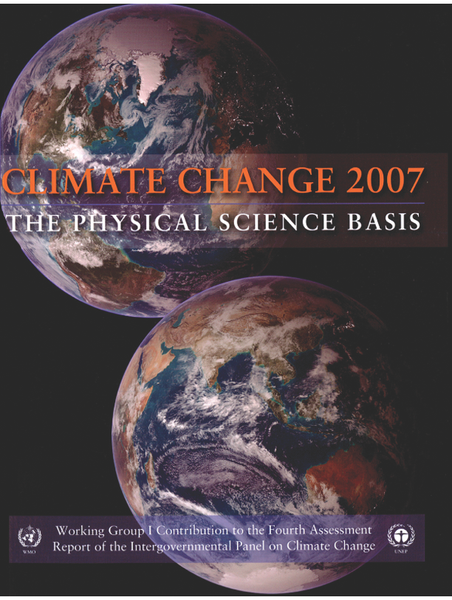
\includegraphics[height=5cm]{ar4-wg1}
      \end{figure}
    \end{column}
    \begin{column}{.5\linewidth}
      \begin{figure}
        
\includegraphics[height=3.5cm]{no-ice-sheet-models}
      \end{figure}
      \begin{itemize}
      \item No results from ice sheet models included due to the models' inability to track recent changes
      \end{itemize}
    \end{column}
\end{columns}
\end{frame}


\begin{frame}{Observed vs simulated flow speeds (2007 model)}
  \begin{columns}[c]
    \begin{column}{.6\linewidth}
    \begin{figure}
      \includegraphics[height=5.75cm]{gris-obs-exp-old}
      \\ \tiny{adapted from Aschwanden, Fahnestock, Truffer (2016) \textit{Nature Comms.}}
    \end{figure}
    \end{column}
    \begin{column}{.4\linewidth}
      \begin{figure}
        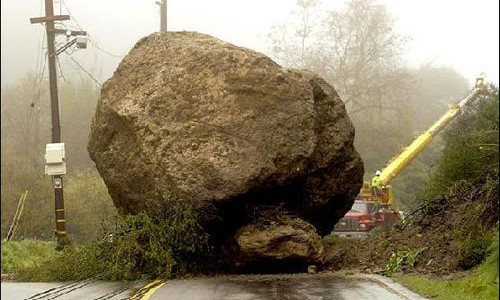
\includegraphics[width=.75\textwidth]{roadblocks}
      \end{figure}
      \begin{itemize}
      \item can't reproduce the velocity field
      \item this led to a model development frenzy
      \end{itemize}
    \end{column}
  \end{columns}
  \note[item]{}
\end{frame}

\begin{frame}{The post AR4 world: Stokes models}
    \begin{figure}
      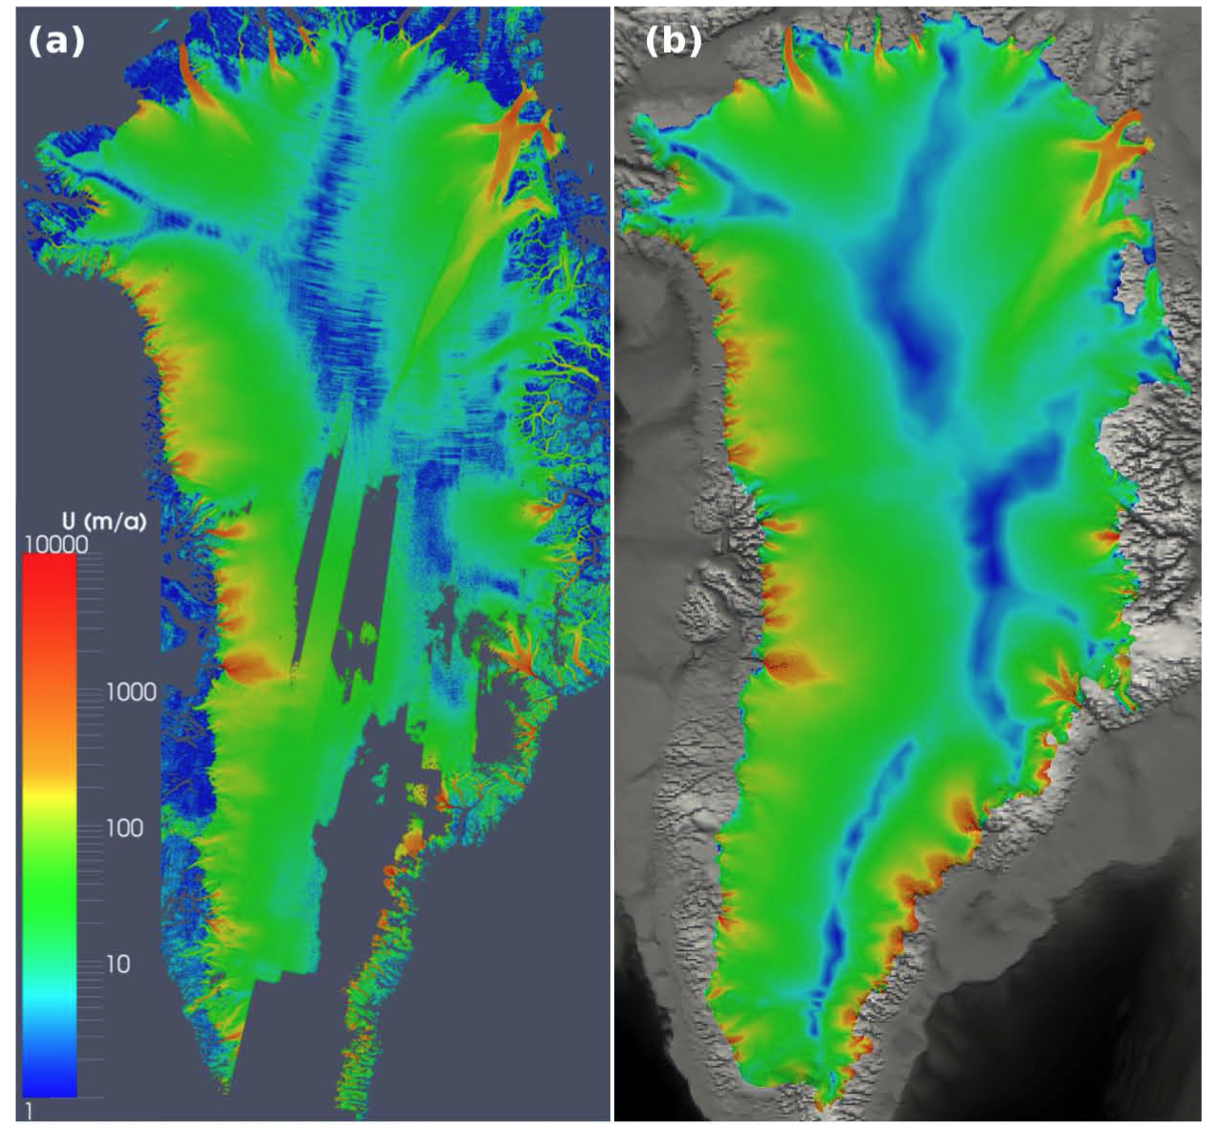
\includegraphics[height=7cm]{gillet-chaulet_2012_fig_1}
      \\ \tiny{Gillet-Chaulet et al. (2012)}
    \end{figure}

\end{frame}

\begin{frame}{The post AR4 world: Sensitivity Analysis}
    \begin{figure}
      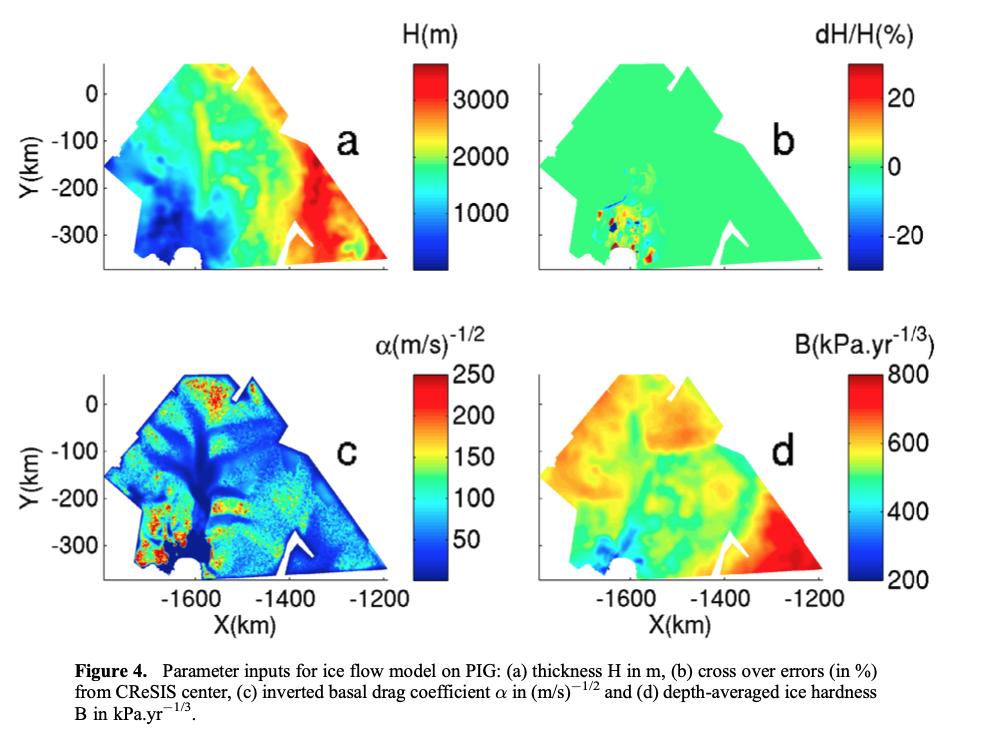
\includegraphics[height=7cm]{larour_2012_fig_4}
      \\ \tiny{Larour et al. (2012)}
    \end{figure}
\end{frame}

\begin{frame}{The post AR4 world: Data Assimilation}
    \begin{figure}
      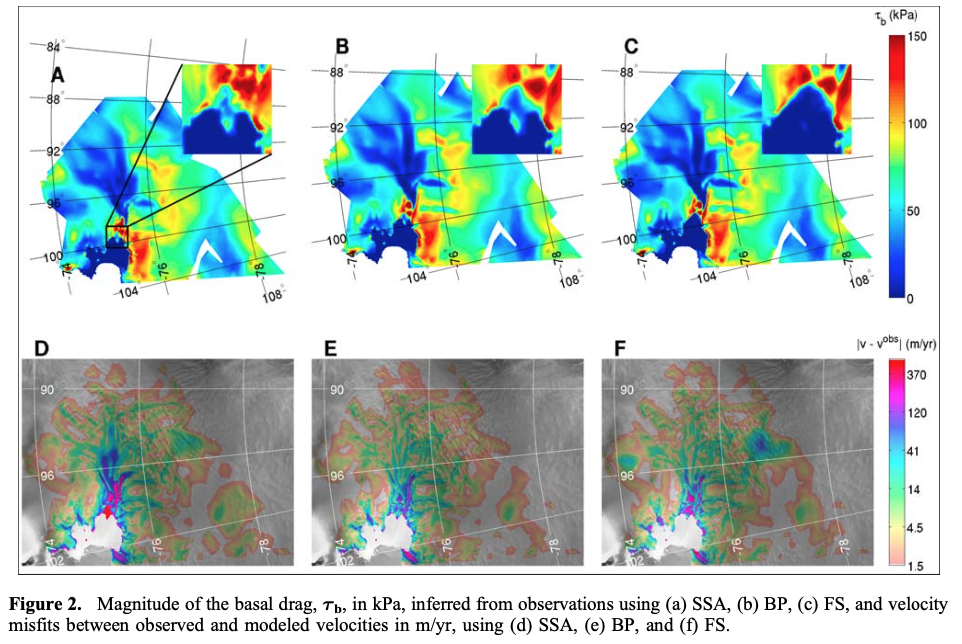
\includegraphics[height=7cm]{morlighem_2010_fig_2}
      \\ \tiny{Morlighem et al. (2010)}
    \end{figure}
\end{frame}

%% \begin{frame}{The post AR4 world: Observations}
%%     \includegraphics<1>[width=.5\textwidth]{world-grace-2002-2016}

%% \end{frame}


\begin{frame}
  \frametitle{IPCC AR5, 2013}
  \begin{columns}[c]
    \begin{column}{.4\linewidth}
      \begin{figure}
        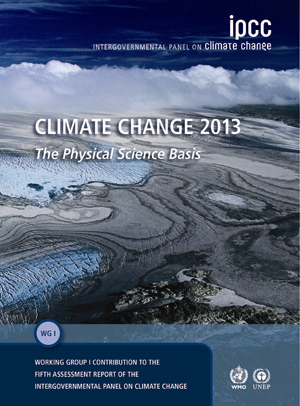
\includegraphics[height=5cm]{ar5-wg1}
      \end{figure}
    \end{column}
    \begin{column}{.6\linewidth}
      \begin{figure}
        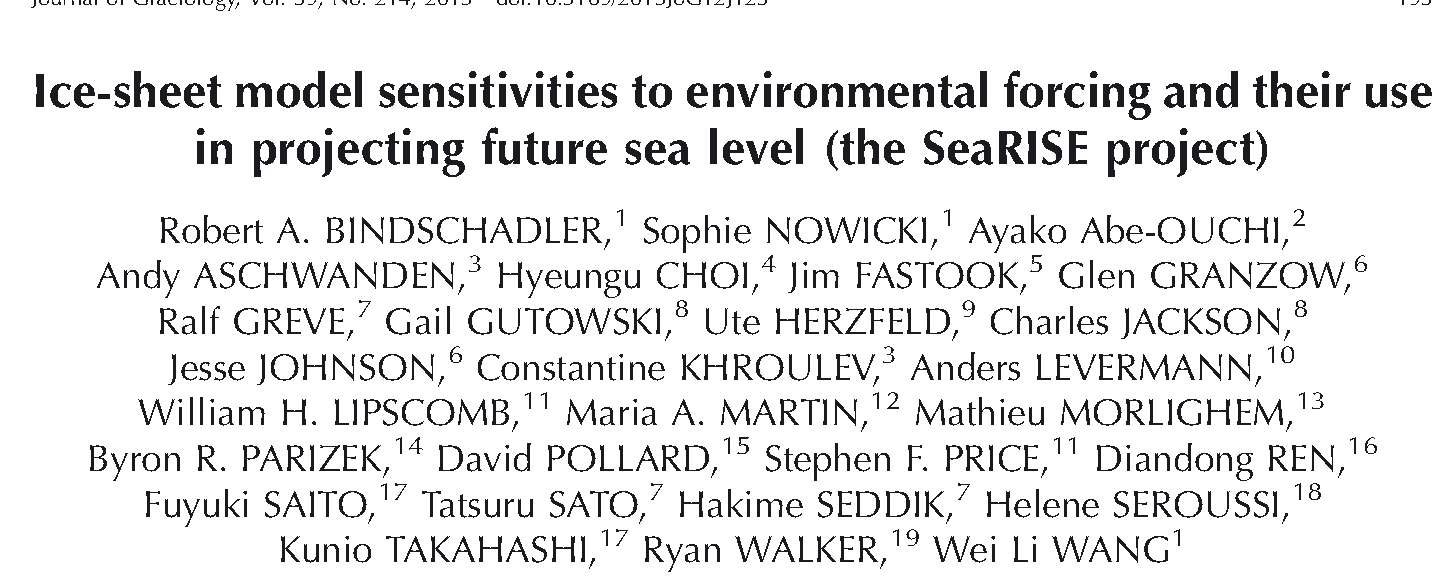
\includegraphics[width=4.75cm]{searise}
      \end{figure}
      \begin{figure}
        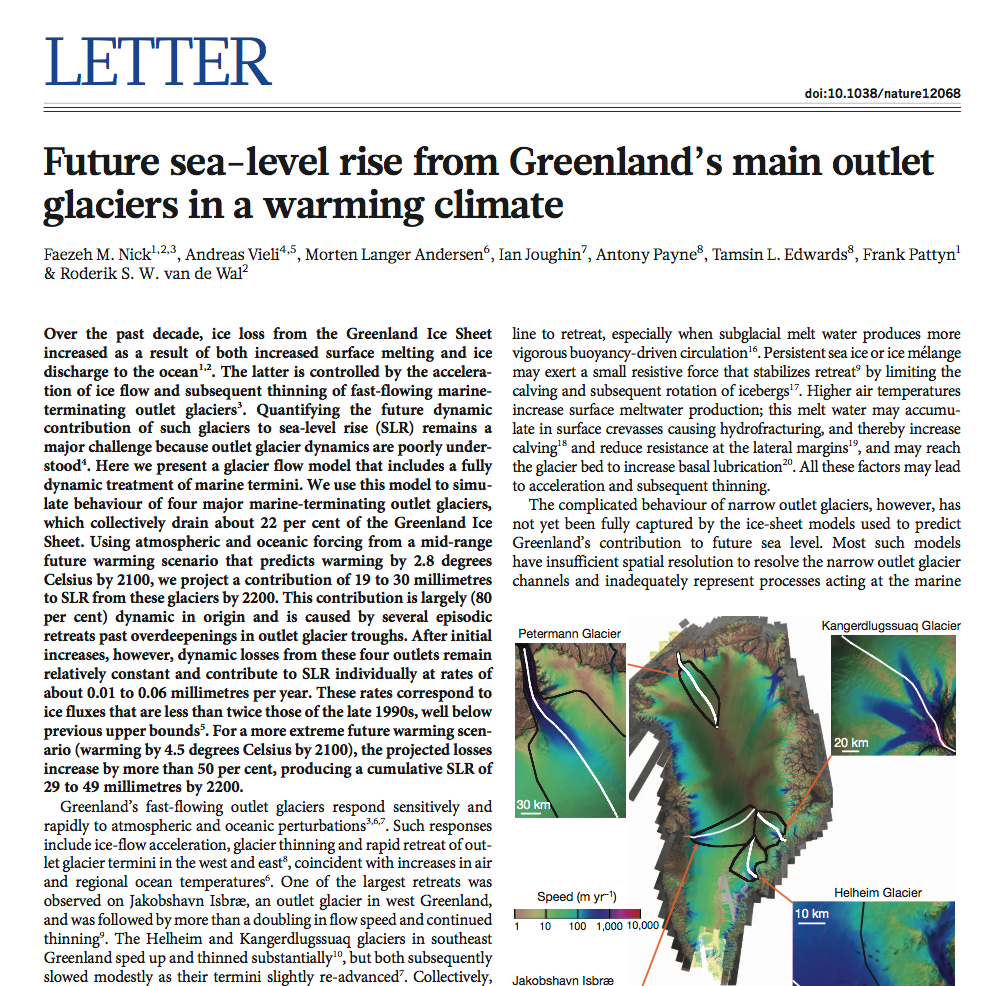
\includegraphics[width=4.75cm]{nick2013}
      \end{figure}
    \end{column}
  \end{columns}
\end{frame}

\begin{frame}{Observed vs simulated flow speeds (2013 model)}
  \alert{Have the models gotten any better? Not really.}
  \begin{columns}[c]
    \begin{column}{.6\linewidth}
    \begin{figure}
      \includegraphics[height=5.75cm]{gris-obs-exp-old}
      \\ \tiny{adapted from Aschwanden, Fahnestock, Truffer (2016) \textit{Nature Comms.}}
    \end{figure}
    \end{column}
    \begin{column}{.4\linewidth}
      \begin{figure}
        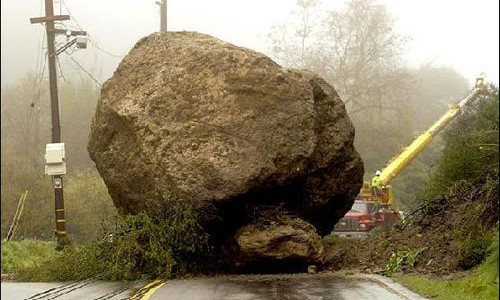
\includegraphics[width=.75\textwidth]{roadblocks}
      \end{figure}
      \begin{itemize}
      \item still can't reproduce the velocity field
      \end{itemize}
    \end{column}
  \end{columns}
  \note[item]{}
\end{frame}

\begin{frame}{Post AR5 models}
  \alert{Have the models gotten any better? Yes.}
  \begin{columns}[c]
    \begin{column}{.6\linewidth}
    \begin{figure}
      \includegraphics[height=5.75cm]{gris-obs-exp-new}
      \\ \tiny{adapted from Aschwanden, Fahnestock, Truffer (2016) \textit{Nature Comms.}}
    \end{figure}
    \end{column}
    \begin{column}{.4\linewidth}
      \begin{figure}
        % 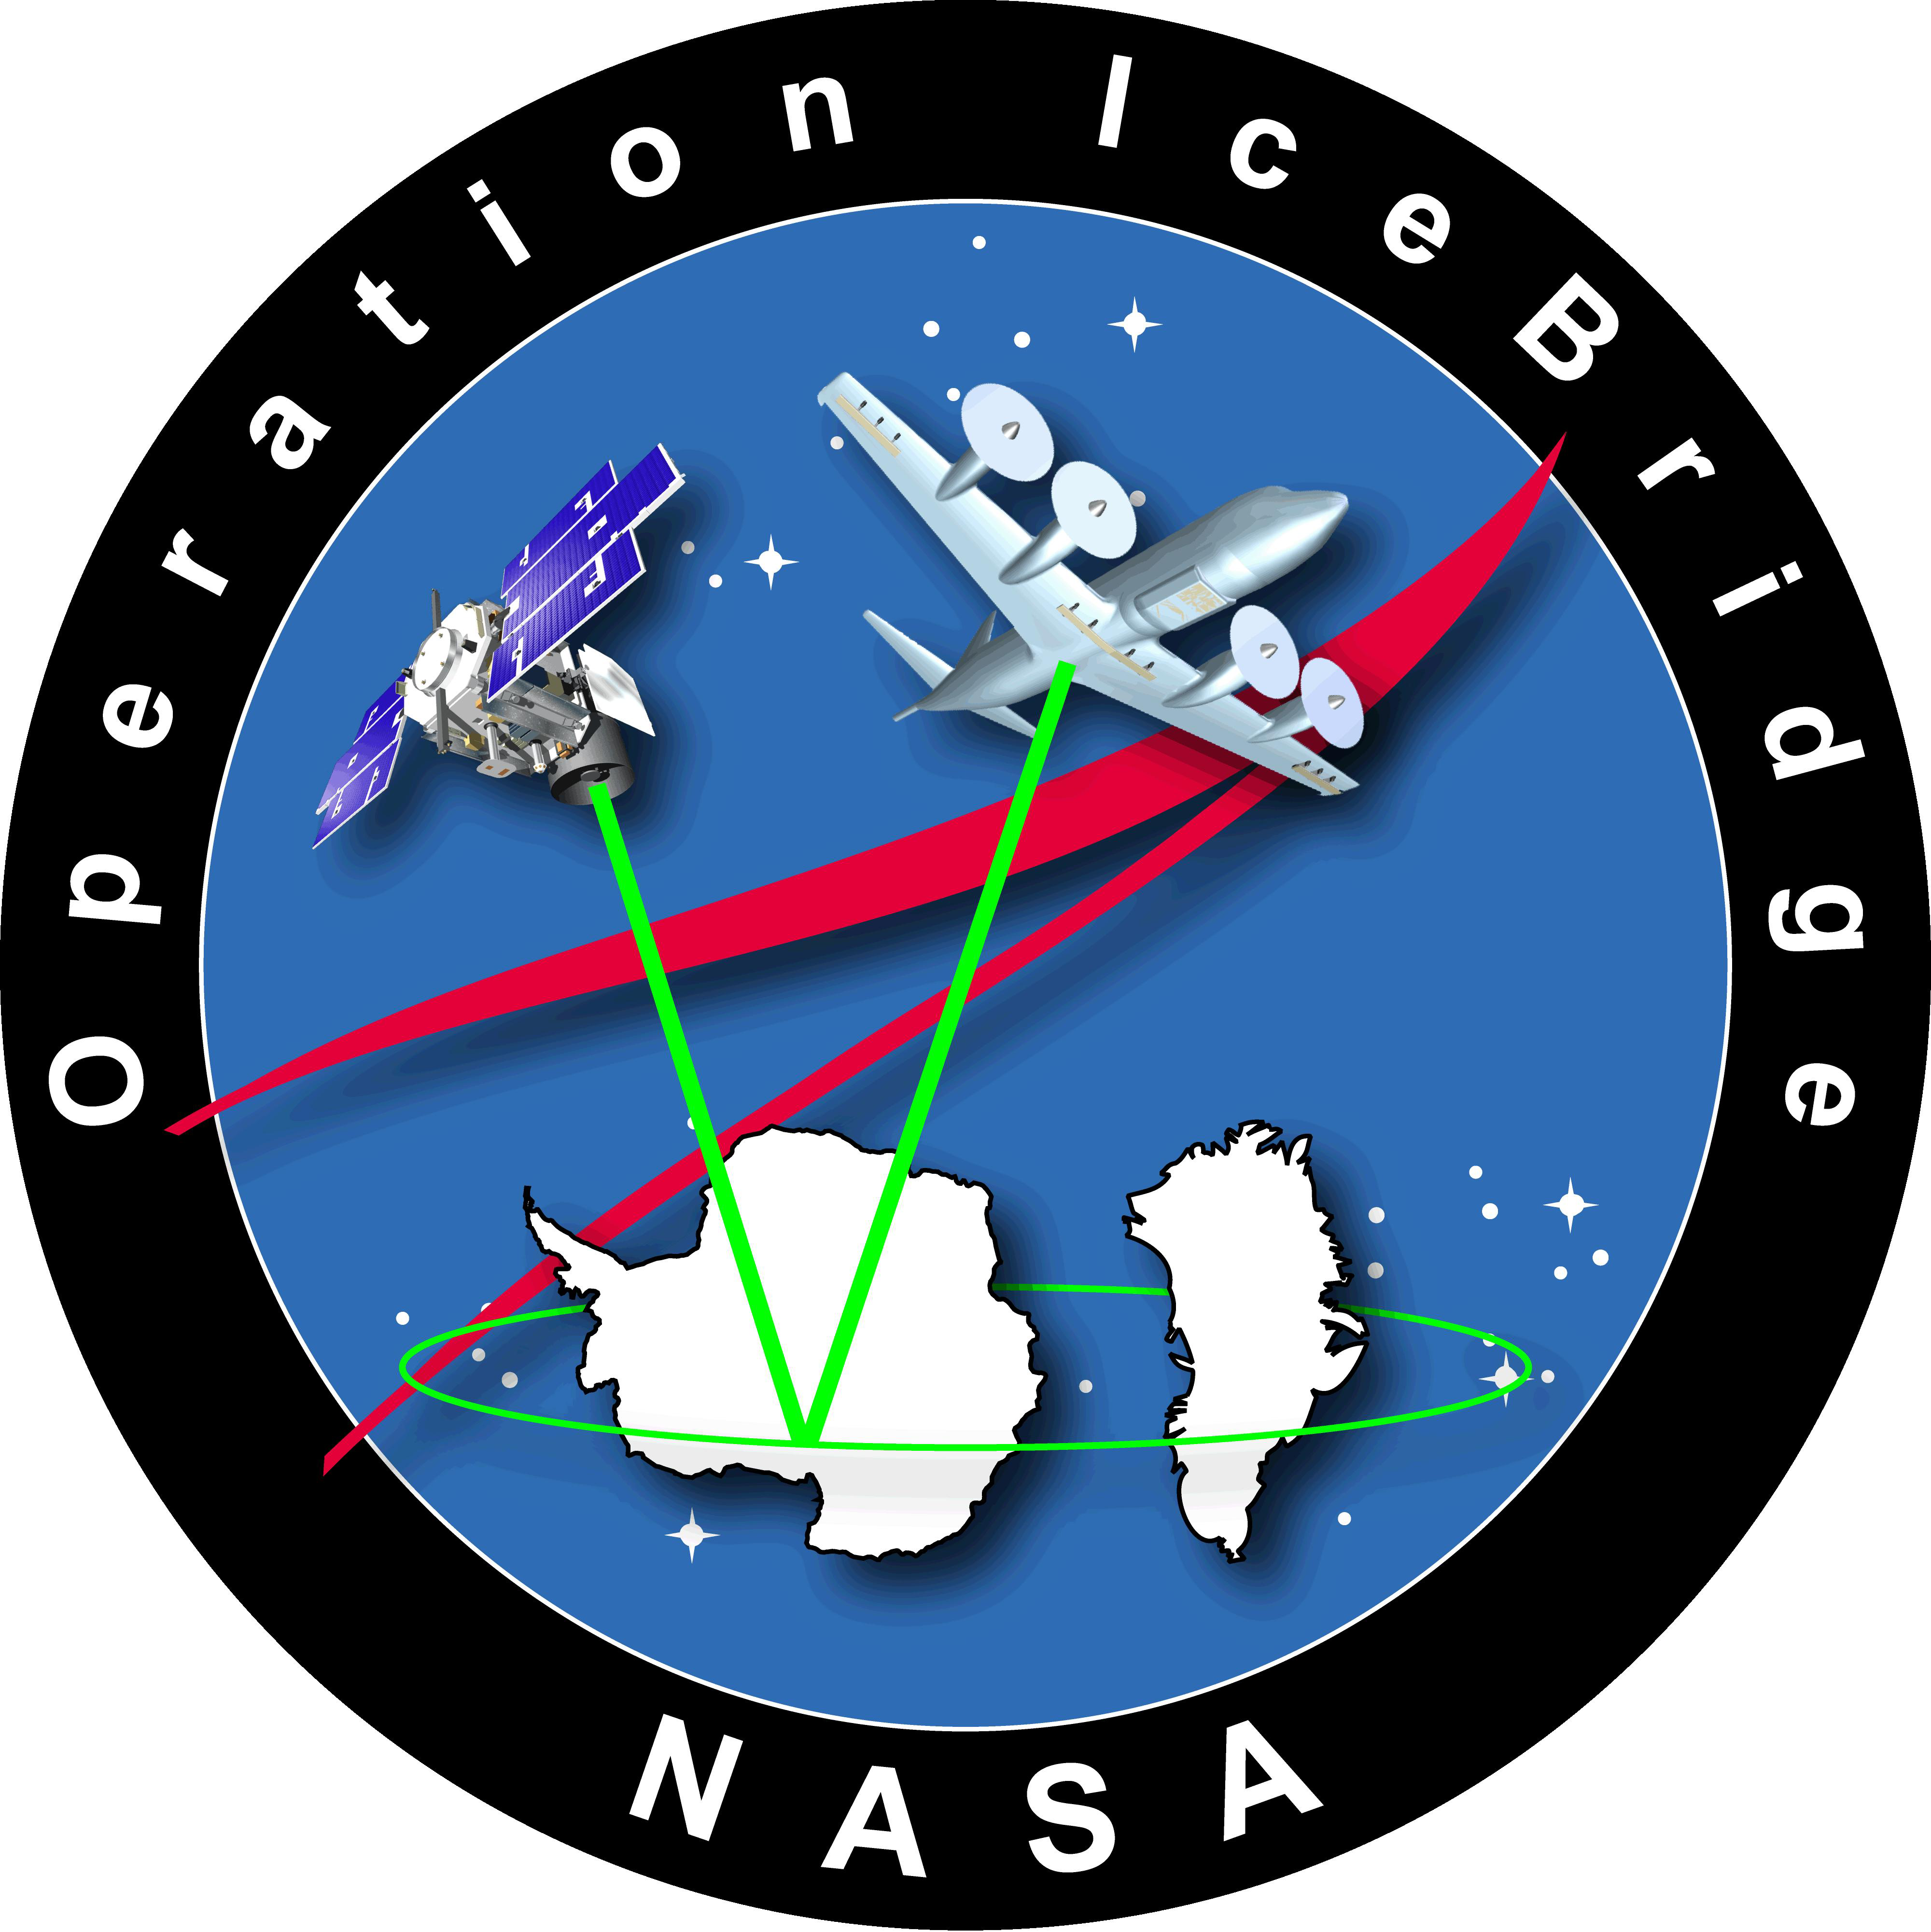
\includegraphics[height=1cm]{oib} \\
        \includegraphics[height=5.75cm]{greenland-bed-mcb}
      \\ \tiny{adapted from Morlighem et al. (2014) \textit{Nature Geosci.}}
      \end{figure}
    \end{column}
  \end{columns}
  \alert{Accurate ice thickness does the trick}
  
  \note[item]{first time capturing the flow field for the right reason}
  \note[item]{this is quite a break through in ice sheet modeling}
  \note[item]{though not a surprising one}
  \note[item]{it just confirms what students learn in glaciology 100:}
  \note[item]{ice flows downhill}
\end{frame}


\begin{frame}
  \frametitle{IPCC AR6, 2021}
  \begin{columns}[c]
    \begin{column}{.4\linewidth}
      \begin{figure}
        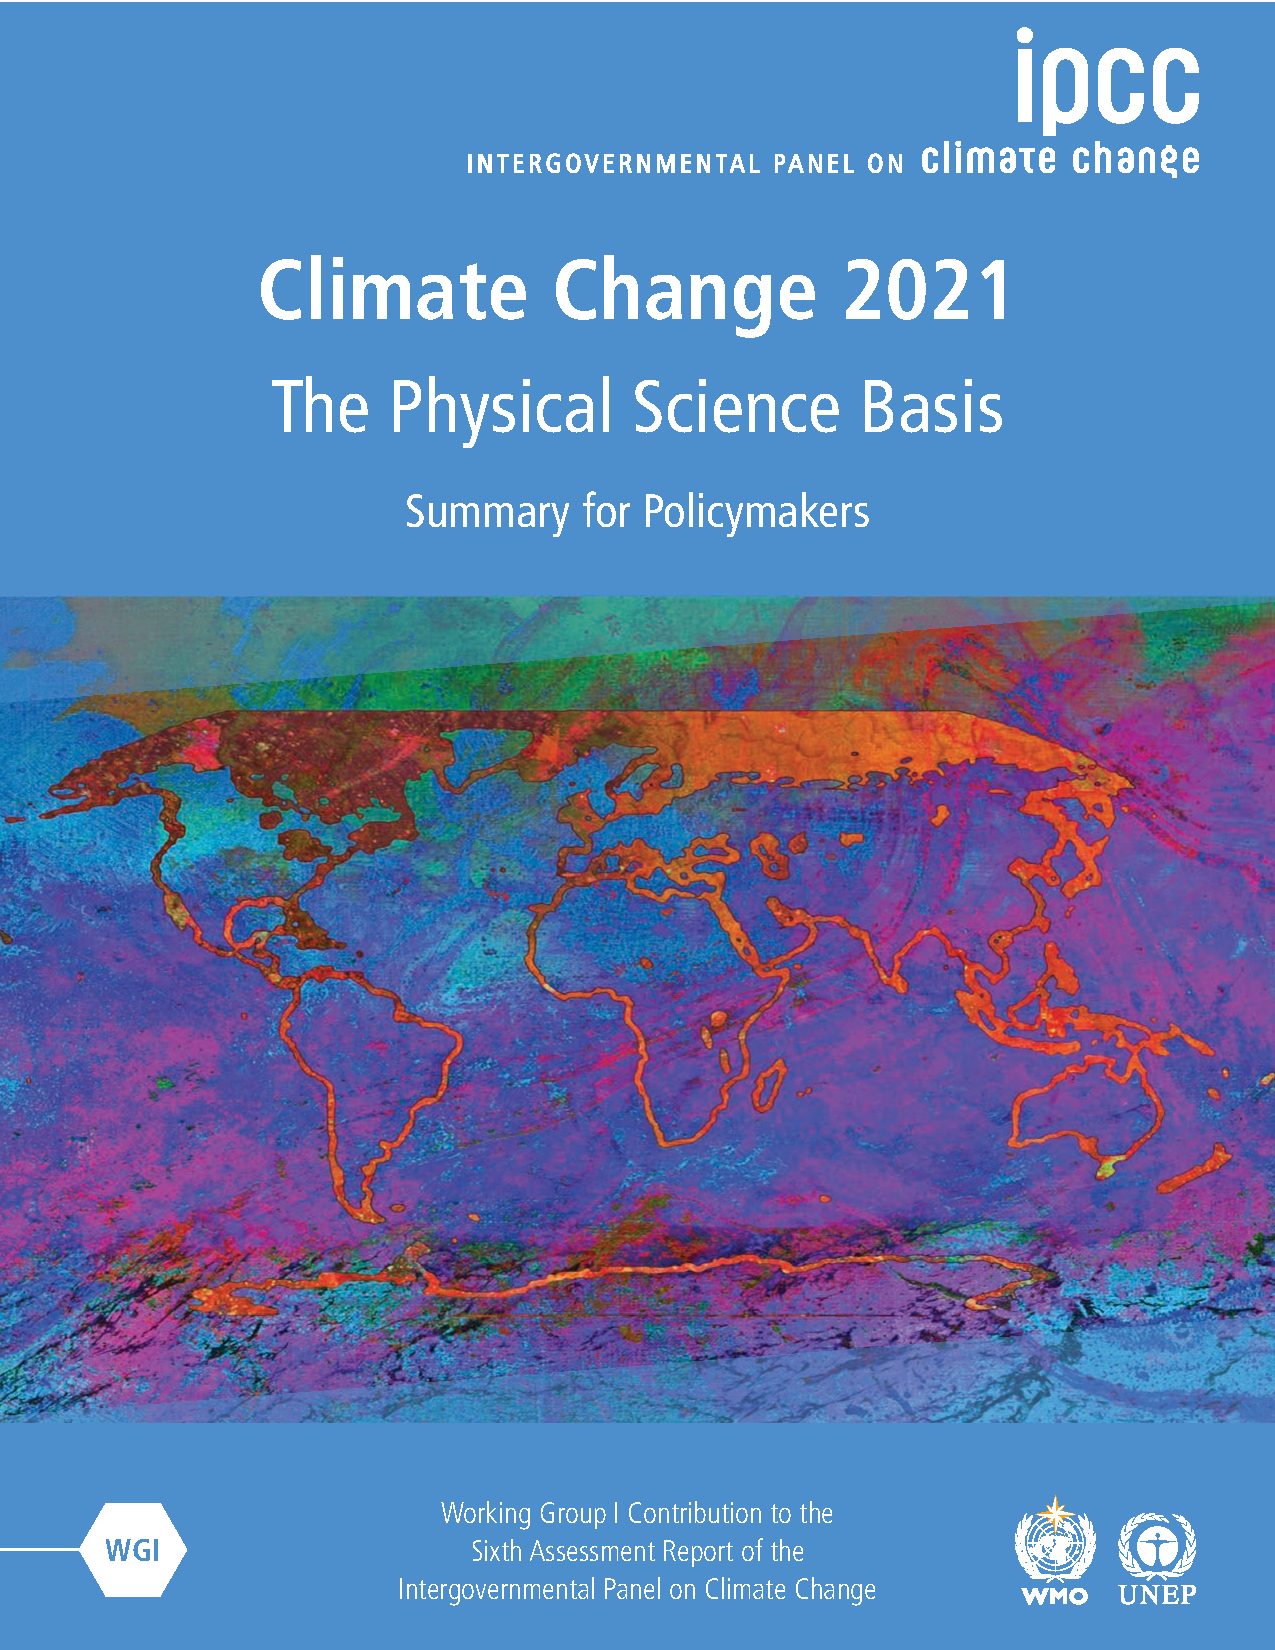
\includegraphics[height=5cm]{ar6-wg1}
      \end{figure}
    \end{column}
    \begin{column}{.6\linewidth}
      \begin{itemize}
      \item multi-model ensemble
      \item Ice Sheet Model Intercomparison Project for CMIP6 (ISMIP6), led by S. Nowicki, H. Goelzer, H. Seroussi, T. Payne and many more
      \item other efforts: ABUMIP, LARMIP-2, MISMIP+, etc.
      \end{itemize}
        \includegraphics<1>[width=2.5cm]{ismip6_logo}
    \end{column}
  \end{columns}
\end{frame}


\part{What's going on?}
\frame{\partpage}

\begin{frame}{A closer look: Greenland}
  \begin{figure}
    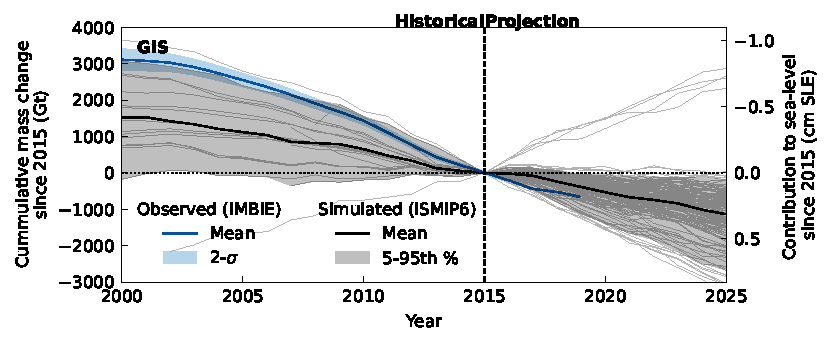
\includegraphics[width=\textwidth]{GIS_historical}
    \caption{Aschwanden, Brinkerhoff, Bartholomaus, \& Truffer (2021)}
  \end{figure}
  \begin{columns}[c]
    \begin{column}{.5\textwidth}
      \begin{minipage}[t][.5\textheight][t]{\textwidth}
        \alert{Almost all historical simulations under-estimate modern mass loss}
      \end{minipage}
    \end{column}
    \begin{column}{.25\textwidth}
    \end{column}
  \end{columns}
\end{frame}

\begin{frame}{A closer look: Antarctica}
  \begin{figure}
    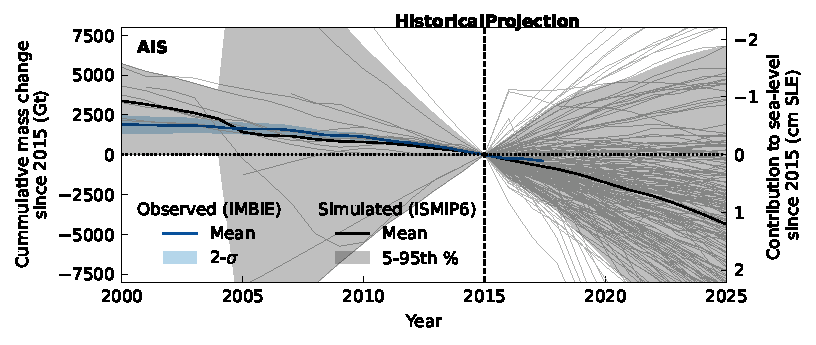
\includegraphics[width=\textwidth]{AIS_historical}
    \caption{Aschwanden, Brinkerhoff, Bartholomaus, \& Truffer (2021)}
  \end{figure}
  \begin{columns}[c]
    \begin{column}{.5\textwidth}
      \begin{minipage}[t][.5\textheight][t]{\textwidth}
        \alert{Spread in simulations much larger than observational uncertainty}
      \end{minipage}
    \end{column}
    \begin{column}{.25\textwidth}
    \end{column}
  \end{columns}
\end{frame}


\begin{frame}{Try it yourself}
  \begin{figure}
    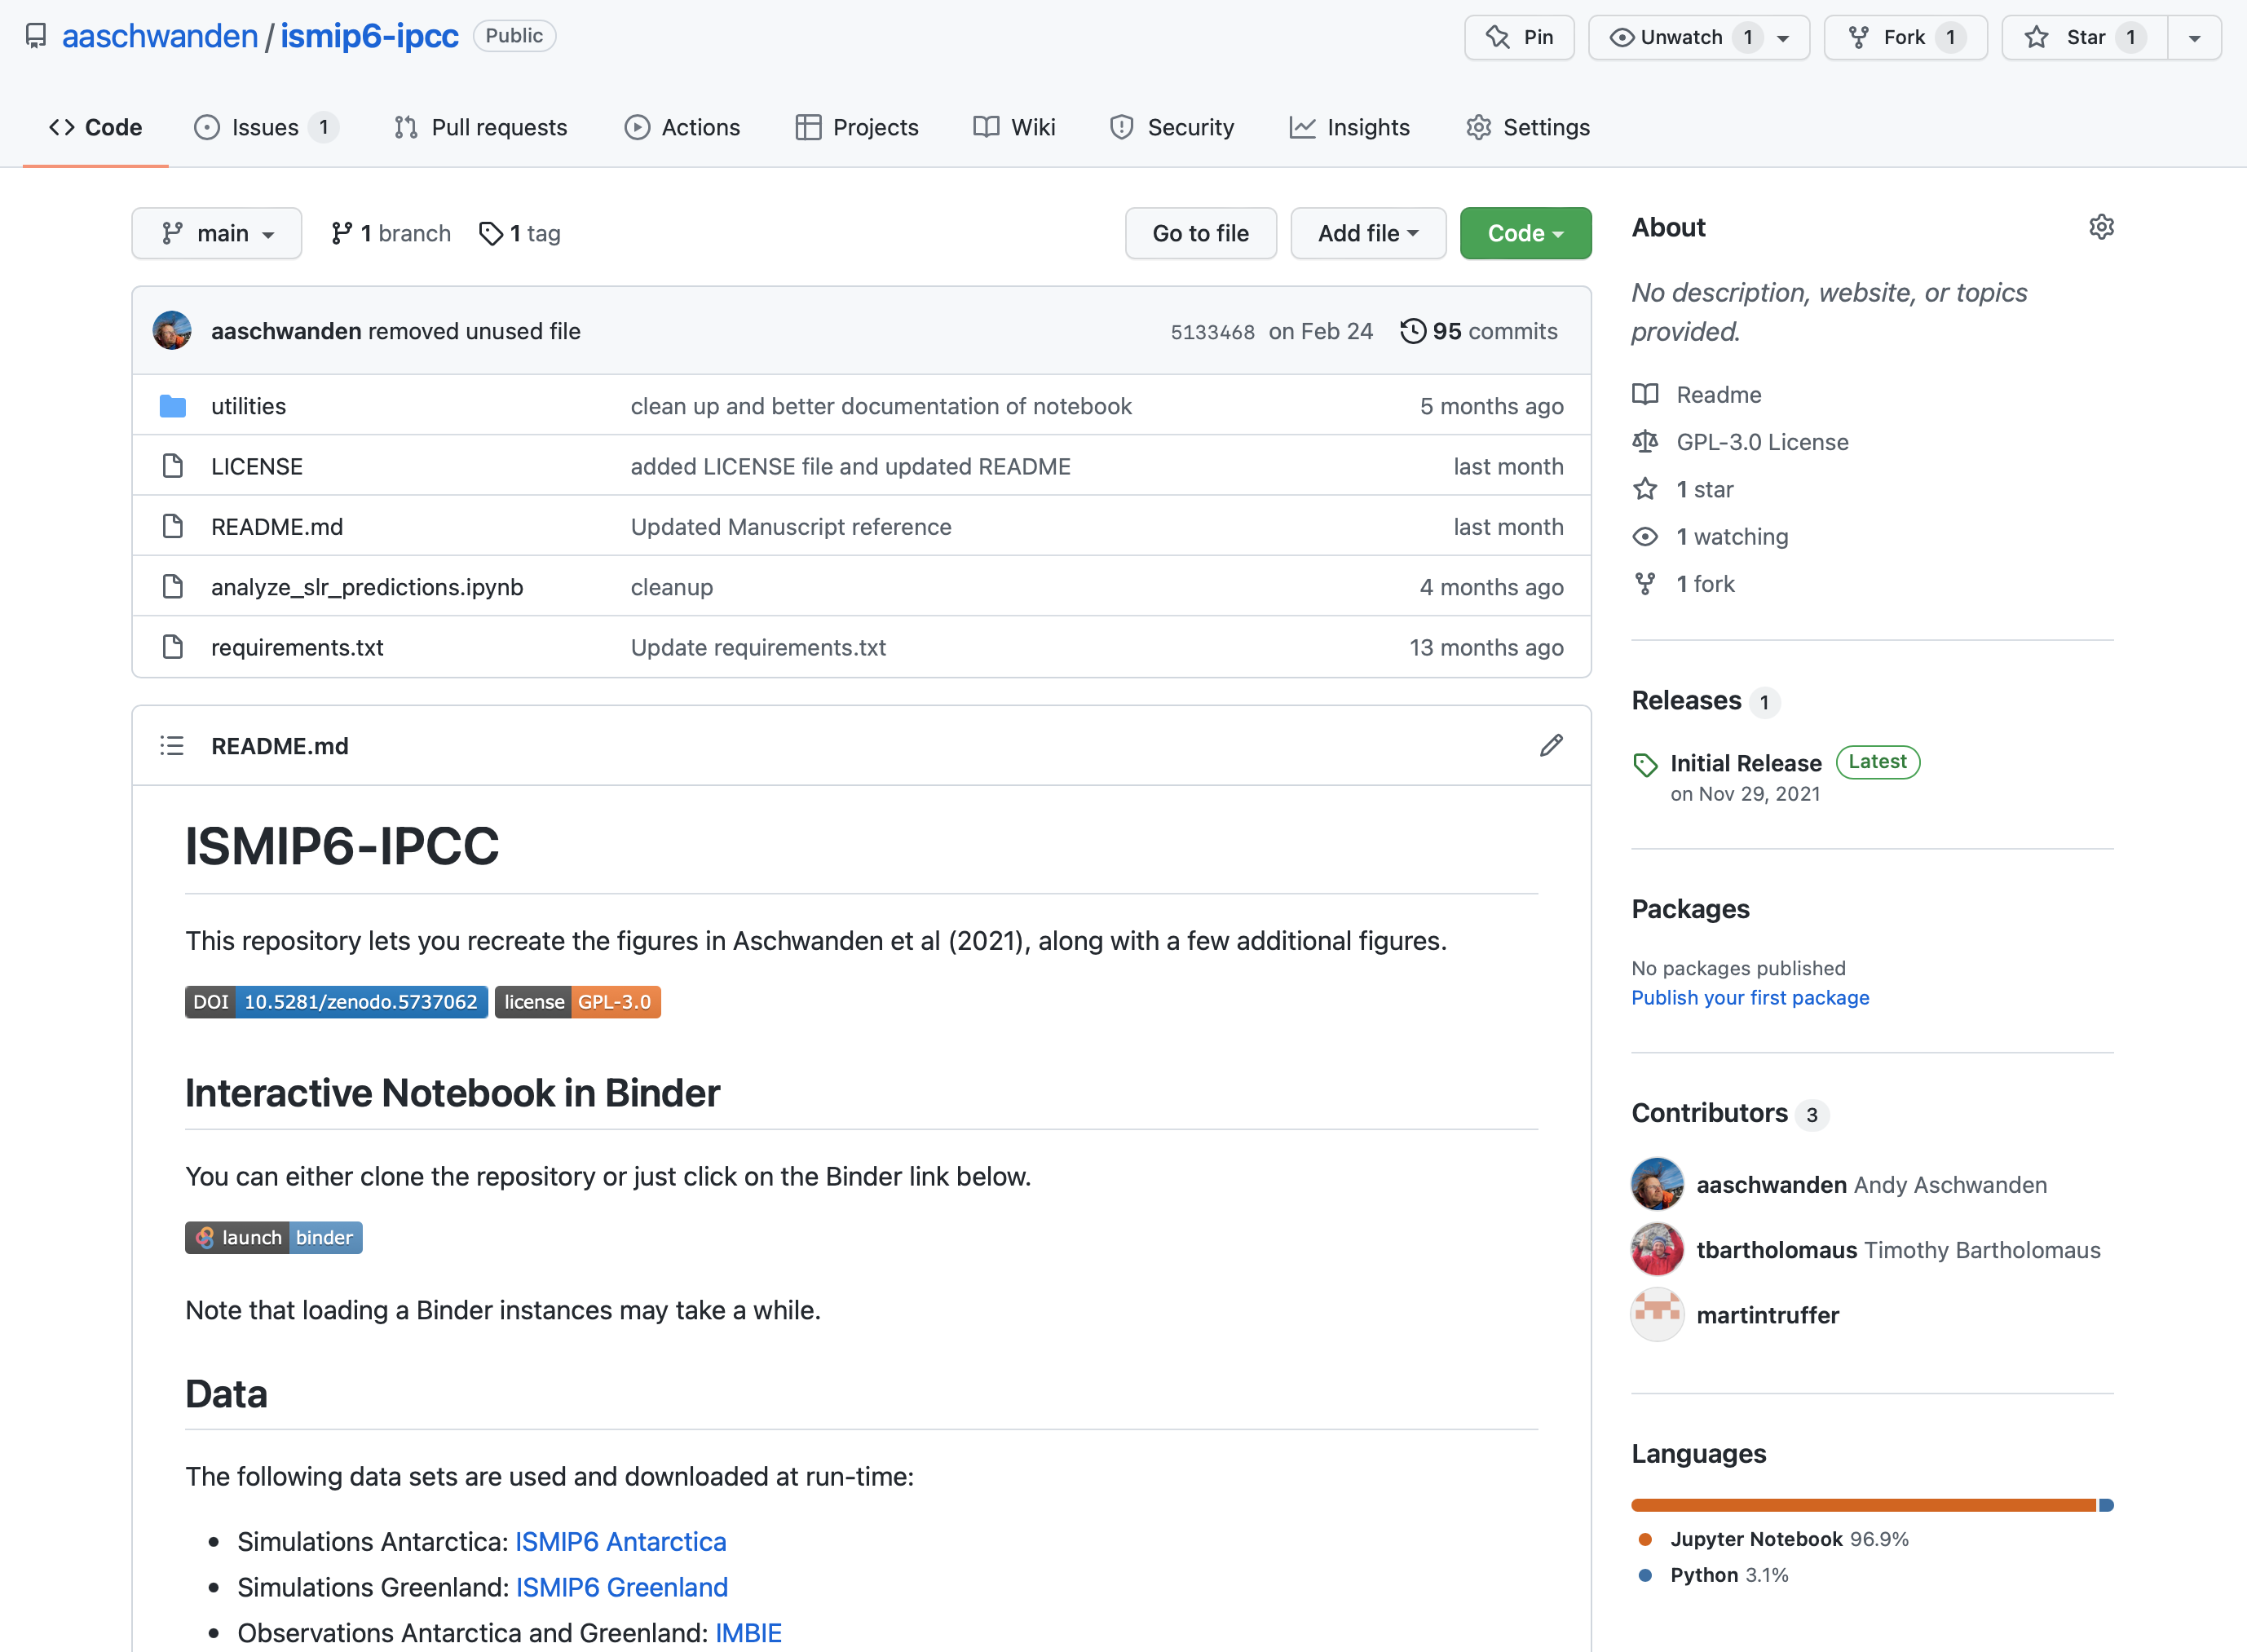
\includegraphics[width=.85\textwidth]{ismip6-ipcc-github-repo}
  \end{figure}
\end{frame}


\setbeamertemplate{background canvas}
  {
     \tikz{\node[inner sep=0pt,opacity=0.35] {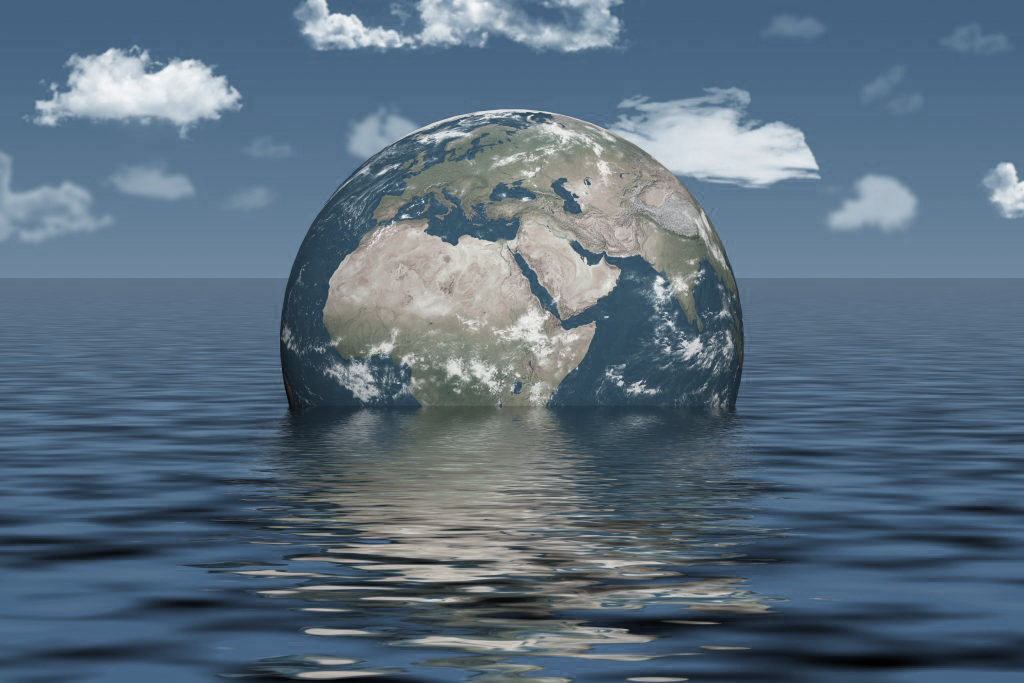
\includegraphics[height=\paperheight]{earth-drowning-desat}};}
}


\part{A path forward}

\frame{\partpage}

\setbeamertemplate{background canvas}
  {
}

\begin{frame}{2 key requirements}
Accurate predictions of the cryosphere's contribution to sea level require that models:
\begin{enumerate}
    \item Fully characterize uncertainties in model structure, parameters, initial conditions, and boundary conditions.
    \item Yield simulations that fit observations within observational uncertainty. 
\end{enumerate}
  \begin{figure}
    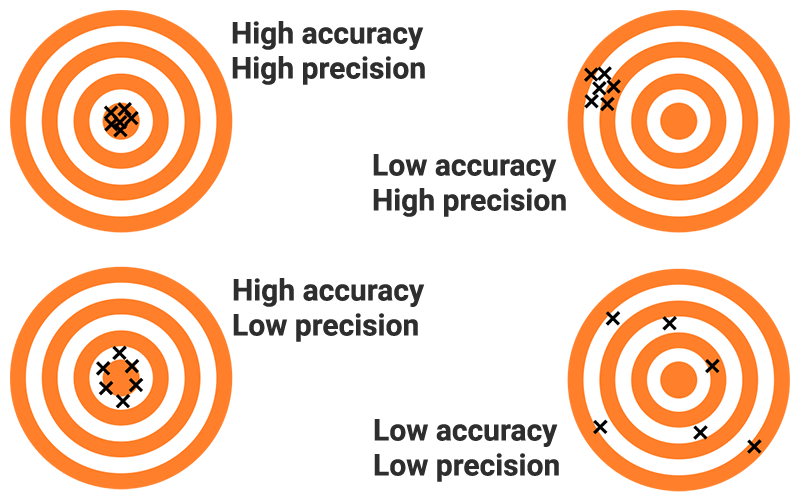
\includegraphics[width=0.4\textwidth]{difference-accuracy-and-precision}
  \end{figure}
  \begin{itemize}
    \item \alert{No new ideas.}
  \end{itemize}
\end{frame}

\begin{frame}{Accounting for all sources of uncertainty}
    \begin{minipage}[t][3.2cm][t]{\textwidth}
    \begin{figure}
      \includegraphics<1->[height=3cm]{sle_pdf_initial}
    \end{figure}
  \end{minipage}
  We can cast this in a \alert{Bayesian} framework:
  \begin{columns}[c]
    \begin{column}{.4\textwidth}
  \begin{itemize}
  \item model uncertainty
  \item inital state uncertainty
  \item parametric uncertainty
  \item aleatoric uncertainty
  \end{itemize}
    \end{column}
    \begin{column}{.55\textwidth}
\begin{align} 
    P(\Delta z|\mathcal{F})&= \int P(\Delta z|f,\mathbf{k},\mathcal{M}) \nonumber \\
                           &  \times P(f|\mathcal{F}) P(\mathbf{k}|\mathcal{M})  P(\mathcal{I}|\mathcal{M})P(\mathcal{M}) \nonumber \\
                           & \times \mathrm{d} \mathbf{k} \; \mathrm{d} f \; \mathrm{d} \mathcal{I}\; \mathrm{d} \mathcal{M}.
    \label{prior_distribution}
\end{align}
    \end{column}
  \end{columns}
  \vspace{1em}
\alert{$\Rightarrow$} Is that the good or the ugly part??

\end{frame}

\begin{frame}{Model uncertainty}
  \begin{figure}
    \includegraphics<1>[width=5cm]{ismip6_logo}
  \end{figure}
  \begin{itemize}
    \item
  \end{itemize}
\end{frame}

\begin{frame}{Initial state uncertainty}
  \begin{figure}
  \includegraphics<1>[width=7cm]{initial-state-ensemble} \\
    \tiny{credit: ECMWF}
  \end{figure}
  \begin{itemize}
  \item time scale when \alert{ice sheet weather} turn into \alert{ice sheet climate} not known (analogy from Vaughan and Arthern, 2007)
  \item perturbation analysis: is ice thickness the analog for sea surface temperature?
  \end{itemize}
\end{frame}


\begin{frame}{Parametric uncertainty}
  \begin{columns}[c]
    \begin{column}{.5\textwidth}
  \begin{figure}
    \includegraphics<1>[width=3cm]{stone_2010_fig_6} \\
    \includegraphics<1>[width=5cm]{stone_2010_fig_7} \\
    \tiny{Stone et al, 2010}
  \end{figure}
    \end{column}
    \begin{column}{.5\textwidth}
  \begin{figure}
    \includegraphics<1>[width=5cm]{bulthuis_2019_fig_6} \\
    \tiny{Bulthuis et al, 2019}
  \end{figure}
    \end{column}
  \end{columns}
\end{frame}






\begin{frame}
  \begin{minipage}[t][3.2cm][t]{\textwidth}
    \begin{figure}
      \includegraphics<1->[height=3cm]{sle_pdf_uq}
    \end{figure}
  \end{minipage}
  Build upon ISMIP6 but each model contributes an ensemble of simulations
  \begin{itemize}
  \item  using random parameter values drawn from consensus estimates of the uncertainties associated with parametrically defined physics
  \item random realizations of climate and ocean forcings
  \item will yield a distribution of sea level projections that is much broader, and thus less certain, than that presented in recent sea level rise projections
  \end{itemize}
\end{frame}

\begin{frame}{Conditioning simulations on observations}
  \begin{minipage}[t][3.2cm][t]{\textwidth}
    \begin{figure}
      \includegraphics<1->[height=3cm]{sle_pdf_calib}
    \end{figure}
  \end{minipage}
    \begin{columns}[c]
    \begin{column}{.45\textwidth}
    \begin{figure}
      \includegraphics<1->[height=3.5cm]{nias_2019_fig_1} \\
      \tiny{Nias et al, 2019}
    \end{figure}
    \end{column}
    \begin{column}{.45\textwidth}
    \begin{figure}
      \includegraphics<1->[height=3.5cm]{gilford_2020_fig_6} \\
      \tiny{Gildford et al, 2020}
    \end{figure}
    \end{column}
    \end{columns}
\end{frame}


\begin{frame}{Bayesian Calibration}
    \begin{minipage}[t][2cm][t]{\textwidth}
      \begin{block}{Which observations should we use?}
        \begin{itemize}
        \item<2-> use the quantity of interest: mass change
        \item<3> use quantity that contributes a lot to uncertainty: ice flow
        \end{itemize}
        \note[item]{}
      \end{block}
  \end{minipage}
    \begin{minipage}[t][6cm][t]{\textwidth}
        \begin{columns}[c]
    \begin{column}{.3\textwidth}
    \includegraphics<3>[height=5.5cm]{greenland-obs-rignot}
    \end{column}
    \begin{column}{.65\textwidth}
    \includegraphics<1->[height=3cm]{GIS_hist_only_obs}
    \end{column}
  \end{columns}

    \end{minipage}

\end{frame}

\begin{frame}
  \begin{figure}
    \includegraphics<1->[height=8cm]{sle_pdf_w_obs_2020_2100}
  \end{figure}
\end{frame}

\part{?}
\frame{\partpage}


\begin{frame}{this comes at a steep cost}
The ambitious characterization of uncertainties and en- semble conditioning we propose requires a massive interna- tional and inter-agency effort in both model development and improved observational capabilities. We call for professional support for the largely computational sea level projection ef- fort. These resources, in the form of dedicated developers and high-performance computing time, will free up scien- tists to continue basic science,
\end{frame}


\begin{frame}
 \frametitle{Lack of funding}
  \begin{columns}[c]
    \begin{column}{.5\linewidth}
      \centering{200M USD}
      \begin{figure}
        \includegraphics[height=5cm]{spiderman-nowayhome}
      \end{figure}
    \end{column}
    \begin{column}{.5\linewidth}
      \centering{$\approx$10M USD per year}
      \begin{figure}
        \includegraphics[height=3.5cm]{nsf_logo_color}
      \end{figure}
      \centering{for glaciology}
    \end{column}
\end{columns}
\end{frame}


\begin{frame}
Funding for glaciological research is tiny compared to the problem at hand
\end{frame}


\begin{frame}{Final thoughts}
  \begin{enumerate}
  \item Fully characterize uncertainties in model structure, \alert{parameters}, initial conditions, and boundary conditions.
  \item \alert{Yield simulations that fit observations within observational uncertainty.}
  \end{enumerate}
  \begin{itemize}
  \item the surrogate model is only used to aid in model calibration
  \item \alert{not} for the actual projections
  \end{itemize}
\end{frame}


\end{document}
